\chapter{刻度}

\section{概述}

刻度设备得出整个$\gamma$能谱测量系统的绝对效率曲线,同时考虑到准直组件和设备在反应堆单元中的物理布局。

在经验方法中,计数效率仅仅只是一个跟光电峰计数率和源强成比例关系,如下所示:
\begin{equation}
\label{eq:equ1}
CR\,=\,EF\,\bullet\,S
\end{equation}
其中,$CR$是计数率,$EF$是光电峰的探测效率,$S$是源强(单位源体积单位时间内发射的光子数)。应该指出,尽管$CR$由通过准直器的光子数决定,但是放射源强度仍然可由整个物体的某个或多个部分适当的表示出来。例如,在热交换器上(详见\ref{section:5_5}),准直器正对着充满放射性管的热交换器的圆锥体部分放射强度与期望的计数率符合。然而,源的强度等于单位时间单位面积的单管放出的光子数。因此,计数效率可表示为:
\begin{equation}
\label{eq:equ1}
EF(\frac{c}{\gamma/cm^{2}})=\frac{CR(counts/min)}{S(\frac{\gamma}{cm^{2}-min})}
\end{equation}
其中,$\gamma$表示发射的光子数,$c$表示被探测到的特定能量的光子数。热交换器上测得的计数率除以效率等于热交换器中放射管源每平方厘米光子发射率。在堆主排气线上,源强可用每分钟每英寸长度所发出的光子数$\gamma/in.-min$。探测系统的效率是关于$\gamma$射线能量的函数。通常,有两种方法确定能量和效率的关系。其一,先用几组不同的已知放射源测量探测器的简单几何模型下的效率曲线,再扣除准直器、距离、屏蔽、以及被观察的实际组件几何形状的影响,即可确定实际的效率曲线。其二,在实际的物理装置上用经验方法确定探测系统的效率。第二种方法相对比较简单且更可靠。然而,我们也使用更基本的近似去检查计算的可靠性。

\section{刻度源}

为了尽可能地模拟实际情况,实验选择直径0.5英寸银质管源,与主热交换器管道的直径相等。

由于$^{110m}$Ag在446.8——1562.2\ keV的能量范围内有多条$\gamma$射线,可便于效率曲线的计算。此外,用ORR的水力传送辐照装置制作这种放射源的代价相对便宜。由于银管对ORR堆的反应性有很大的影响,所以一般只有低2.3英寸长的管子才能用此装置进行辐照。因此,本实验分三次辐照此长度的银管。辐照样品前,先用注量监测片(Co-Al片)测量辐照位置的注量率和总注量。辐照之后在热室中处理样品,把这三个管源用不锈钢薄片包裹衔接起来(如图\ref{Fig_5_1})。附件B对源强和源各个位置活度变化率的计算做详细介绍。

\begin{figure}
\centering
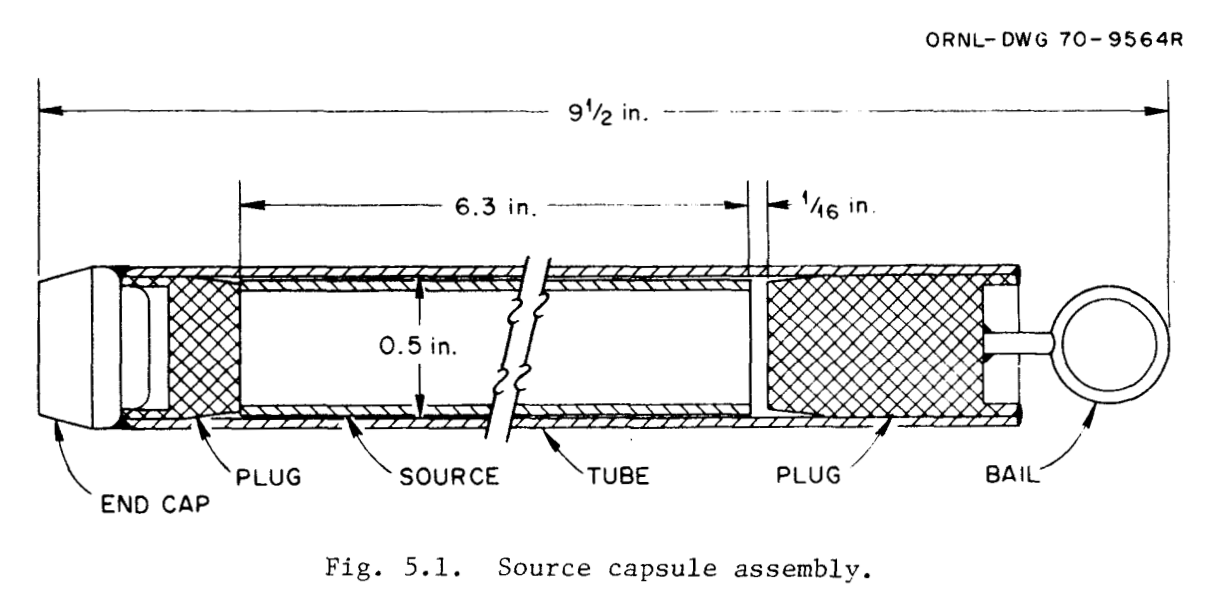
\includegraphics[width=0.8\textwidth]{Fig_5_1}
\caption{Source capsule assembly.}
\label{Fig_5_1}
\end{figure}

\section{狭缝实验——放射源强度}

由于ORR堆中的中子通量分布各异,导致管源在长度上的活化率不一。为了正确刻度探测系统,就必须知道管源活化率的情况。起先,计划通过测量管源上各点$^{110m}$Ag的活度和通量监测片上获得的活化率来推算$^{110m}$Ag的放射性水平(附录B中的表B.2和B.4)。然而,这样处理有很多不确定性。一个更好的处理方法是使用Ge(Li)探测器和准直器区扫描管源。在MSRE的远程维护间(RMPC)中用铅砖堆出一个高两英尺的狭缝,缝宽1/8英寸;一个管源能顺利穿过的玻璃管紧挨着垂直固定在狭缝上。探测器放置在隔壁的去污间,并紧挨在正对狭缝的小孔上。当放射源置于玻璃管之中时,银管1/8英寸处的$\gamma$射线能穿过狭缝、墙体的小洞和准直器,并打到探测器。把源降到狭缝下面,然后开始扫描探测,逐渐提高放射源,直到探测器示意到源的顶部在缝的前面。

在扫描时,以1/8英寸的步长向上移动源并获取相应的$\gamma$能谱,直到整个源都通过狭缝。解谱并画出源位置与光电峰净面积的曲线关系即可得到源的放射性强度的分布轮廓(见\ref{Fig_5_2})。由这些结果可以计算沿管源轴向方向上任何一点的绝对活度(见附录B)。

由于管状银源的活度分布不是完全的均匀,准直器要指向管源有意义的部位,所以计算源强的平均值对于系统来说是十分必要的。源强平均值$\overline{S}$可表示为:
\begin{equation}
\label{eq:equ3}
\overline{S}=\frac{\int_{0}^{L} S(x) R(x) dx}{\int_{0}^{L} R(x) dx}
\end{equation}
其中,$L$为管的长度,$S(x)$为$x$点的源强,$R(x)$为加权函数相当于轴向计数效率(点源的灵敏度响应函数即为源到准直器轴向的距离函数)。在狭缝实验中发现源强$S(x)$和计数率$CR(x)$呈线性相关,因此,式\ref{eq:equ3}可写为:
\begin{equation}
\label{eq:equ4}
\overline{S}=\frac{k \int_{0}^{L} CR(x) R(x) dx}{\int_{0}^{L} R(x) dx}
\end{equation}
其中,$K$是$S(x)$相对于$CR(x)$的比例常数。注意在狭缝实验设置中$K$为源的计数效率的倒数,其单位为(y/in.)/c.。由此可得:
\begin{equation}
\label{eq:equ5}
\overline{CR}=\frac{\overline{S}}{K}=\frac{\int_{0}^{L} CR(x) R(x) dx}{\int_{0}^{L} R(x) dx}
\end{equation}
其中,$\overline{CR}$为整个源管对应的某一$\gamma$射线的平均计数率。

为了确定权重函数$R(x)$,假设准直探测器组件具有旋转对称性;也就是 说,只能从准直轴方向做径向移动。(这个假设要求准直器的小洞要非常直,这看起来是有道理的,至少对1/8英寸的准直器来说。)

在热交换器模型的刻度工作(看\ref{section:5_5})中,可以测量探测器对源从准直器轴的左边到右边的计数率的分布贡献。图\ref{Fig_5_3}为探测器对银管源的轴向各点的归一化灵敏度曲线图。此图由如下数据构成:在热交换器模型的每列管的放射性管源位置上测出$^{110m}Ag$的三个不同光电峰的净计数率(平行于准直轴,如\ref{Fig_3_5})。概括整列的读数的原因是为了获得一个更统一的放射源分布,以及更好的计数统计。通过这个模型的计数率分布,归一三个光电峰到某个统一的值,且纠正准直器的轻微错位。图\ref{Fig_5_3}显示三条归一化曲线的平均值,这个平均值的偏差很小。这幅图也代表了权重函数$R(x)$。乘以管的计数率所得的结果就是探测系统中所看到的源的总有效活性,该计数率通过狭缝实验\ref{Fig_5_2}得到,符合探测器中所看到的归一分布规律。管源选择的三个能量峰的平均计数率等于图\ref{Fig_5_4}中对应的三个面积分别除以图\ref{Fig_5_3}中归一曲线下的面积。我们得到的三个源的加权后的计数率:

%\begin{table}
%\centering
\begin{tabular}[c]{ccc}
\hline
Energy (keV)  &  Count rate (counts/min) \\
\hline
657.7  &  27,500  \\
884.7  &  24,300  \\
937.5  &  13,600  \\
\hline
\end{tabular}
%\end{table}

知道了在不屏蔽条件下这三个能量峰的平均计数率,只需要计算$k$\ 就能确定源的平均强度。

\begin{equation}
\label{eq:equ6}
k_i(x)=\frac{S(x))}{CR(x)}
\end{equation}
$S(x)$\ 与$CR(x)$\ 分别为源在点$x$处的强度和对应的计数率,这些值在狭缝实验中测到。下标i表示第i条$\gamma$\ 射线。既然知道源中两个点的强度(看\ref{Fig_5_2}和附件B),既可以使用狭缝实验得到的结果来计算三条$\gamma$\ 射线在这两点上的$k$。如下所示:

\begin{table}
\centering
\caption{Count rates measured at two positions along the silver source for 	three different photopeaks}
\begin{tabular}[c]{cccccc}
%\caption{Count rates measured at two positions along the silver source for 	three different photopeaks}
\hline
%Photon  &  Count rate from & & Count rate from & \\
%energy &	slit experiment &   $k$(x10$^4$) &  slit experimen & $k$(x10$^4$) 
%&   $\overline{k}$ (x10$^4$) \\
%	&for 3.861 Ci/in.   &    &  for 4.196Ci/in. \\

%\tabincell{c}{Photon \\ energy} & \tabincell{c}{Count rate from \\ slit 
%	experiment \\ for 3.861 Ci/in.  } & $k$(x10$^4$) & \tabincell{c}{Count rate from \\ slit 
%	experiment \\ for 3.861 Ci/in.} &  $k$(x10$^4$) & $ \overline{k}$ (x10$^4$)  \\

\multirow{3}{2cm}{Photon energy} & \multirow{3}{3cm}{Count rate from  slit 	experiment for 3.861 Ci/in.} &  \multirow{3}{2cm}{$k$(x10$^4$)}& \multirow{3}{3cm}{Count rate from  slit experiment  for 3.861 Ci/in.} & \multirow{3}{2cm}{$k$(x10$^4$)}&  \multirow{3}{2cm}{$\overline{k}$ (x10$^4	$)} \\
%& &$k$(x10$^4$) &  & $k$(x10$^4$) &  $ \overline{k}$ (x10$^4$) \\
\\
\\
(keV)& (counts/min) & $\frac{Ci/in. }{counts/min}$  & (counts/min)  & 
$\frac{Ci/in.}{counts/min}$ &   \\
\hline
657.7  &  25,900  &1.491  &28,300  &1.481  &1.486  \\
884.7  &  23,100  &1.675  &25,100  &1.671  &1.673  \\
937.5  &  12,700  &3.044  &14,700  &2.861  &2.953  \\
\hline
\end{tabular}
\end{table}

列出管源上标定位置点上对应的$\gamma$\ 射线的计数率和$k$\ 。此外,也列出管上两点的$k$\ 平均值。通过这些$k$\ 的平均值乘以上面列出的三条$\gamma$\ 射线对应的平均计数率,即可算出源的三个平均强度。计算结果如下:

%\begin{table}
%\centering
\begin{tabular}[c]{ccc}
\hline
Energy (keV)  &  Source strength (Ci/in.) \\
\hline
657.7  &  4.09  \\
884.7  &  4.07  \\
937.5  &  4.00  \\
\hline
\end{tabular}
%\end{table}

由此可算得管源的平均强度为4.05\ Ci/in. 
。

由于使用平面源(源置于热交换器模型内各个位置)去估计线源的权重因子,因此,此类源评估方法过于理想,具有一定的误差。然而,归一化权重曲线\ref{Fig_5_3}两边急剧上升,中间源活度变化平稳,因此,此方法应该是可行的。考虑到评估源的放射性强度和权重因子的误差,估计计算源强度的误差在$\pm5\%$。

\begin{figure}
\centering
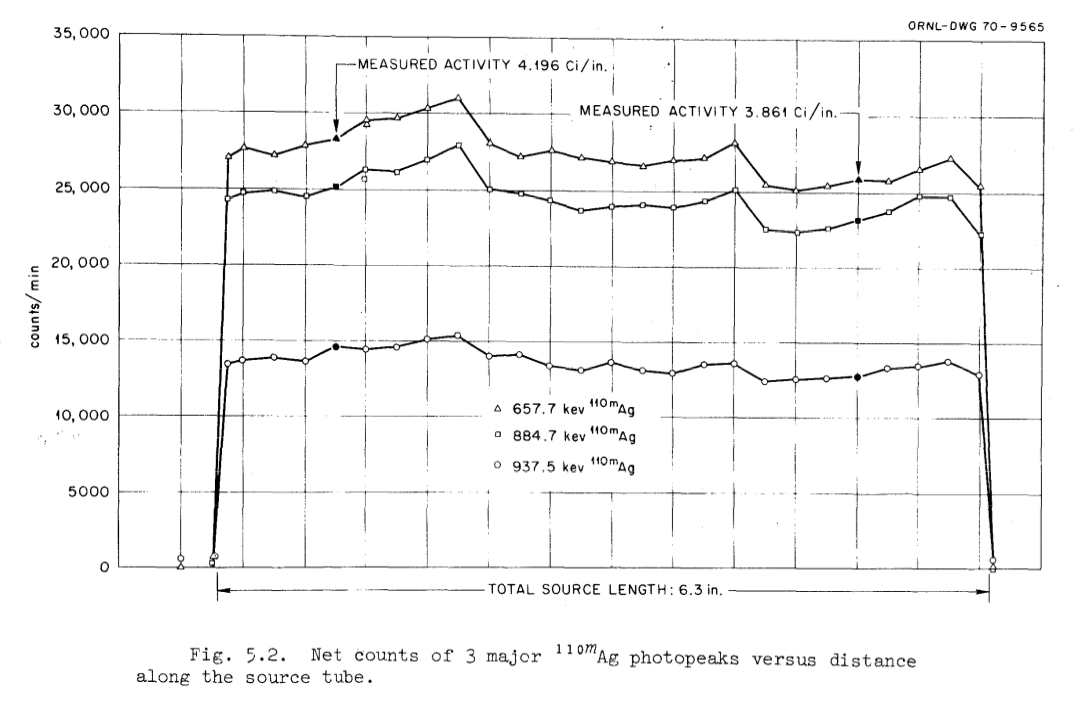
\includegraphics[width=0.8\textwidth]{Fig_5_2}
\caption{Net counts of 3 major $^{110m}$Ag photopeaks versus distance along the source tube.}
\label{Fig_5_2}
\end{figure}

\begin{figure}
\centering
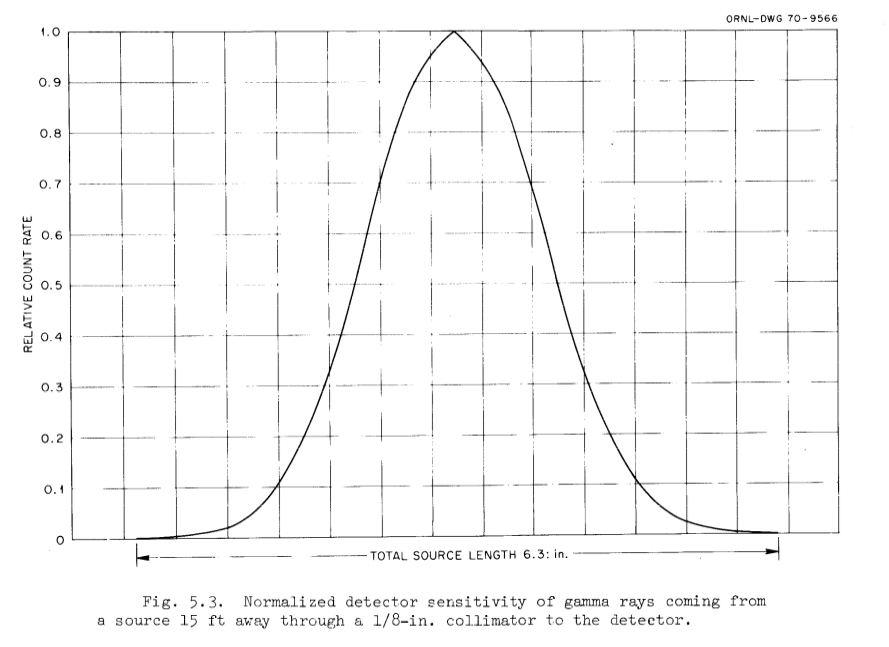
\includegraphics[width=0.8\textwidth]{Fig_5_3}
\caption{Normalized detector sensitivity of gamma rays coming from a source 15\ ft away through a 1/8-in. collimator to the detector.}
\label{Fig_5_3}
\end{figure}


\begin{figure}
\centering
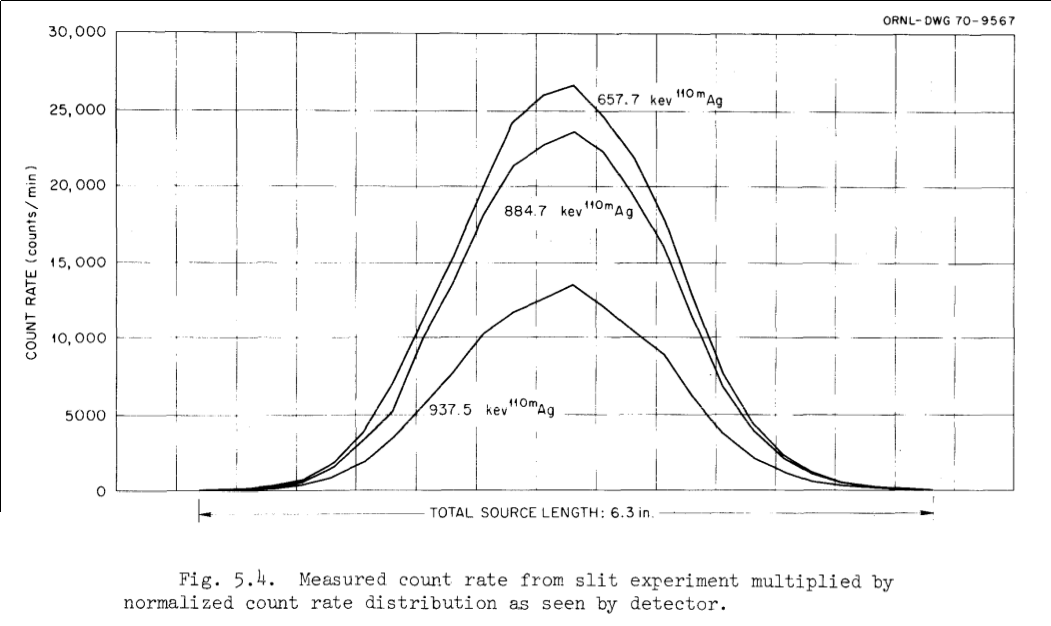
\includegraphics[width=0.8\textwidth]{Fig_5_4}
\caption{Measured count rate from slit experiment multiplied by normalized count rate distribution as seen by detector.}
\label{Fig_5_4}
\end{figure}

\section{单放射源实验}

单源实验是为了刻度用于测量反应堆中主排气线的$\gamma$\ 射线的探测系统的效率。假设探测器对$^{110m}$Ag管源和直径1英寸的折叠主排气线有相同的计数效率。管源安装在未屏蔽的热交换器模型的中心位置, 准直器由激光校准。微调准直器使得设备获得最大的计数率。管源到探测器的距离大约等于PMS上的探测装置到堆单元中的主排气线的距离。使用$1/8$英寸内径的准直内插件。

依据实验获得的数据和不同$\gamma$\ 射线($^{110m}$Ag的15个光电峰)的绝对分支比,我们能算出探测系统在这些能量点上探测效率。用$^{110m}$Ag的446.8keV到1562.2keV的$\gamma$\ 射线估计出探测器的绝对效率曲线。由于很多裂变产物的光电峰不在此能量范围内,所以需要扩展效率曲线去突破这些限制。决定使用从排气线上获得的裂变产物谱来扩展效率曲线的能量范围。例如,使用$^{99}$Mo,$^{131}$I,$^{132}$I和$^{140}$La的140到2522keV能量点作出相对效率曲线。再匹配$^{110m}$Ag的绝对效率曲线,即可获得一条宽能量范围的绝对效率曲线。图\ref{Fig_5_5}为堆内排气线采用的效率曲线。

同时使用光电峰超出能量范围的$^{226}$Ra源去检查上面的方法。此源得到的相对效率曲线的形状基本上与绝对效率曲线的一样。它们的差异可能是由于实际发射光子对屏蔽的不同表现引起的,在低能端尤其明显。


\section{热交换器刻度}\label{section:5_5}

热交换器刻度是通过热交换器模型的整体尺寸进行刻度。8.5英寸长的模型管子的外直径和壁厚与实际的热交换器管子一样。在模型中,这些管被垂直固定在两个相距约6英寸水平板上,且以边长为0.775英寸的正三角形排列。借助简单的工具,可以容易在PMS上的操作孔中操控这些管子。这个模型包含20行管子(与探测器准直器轴向垂直)。由于呈正三角形排列,每行有八或九个管子。为了模拟热交换器的壳层,在模型前面适当位置放置一个厚0.5英寸的不锈钢曲面。

在这个模型中任选某个管位插入一个放射性管源,其他所有管位用仿造管代替,然后进行采谱。这样操作进行两遍,一次用4400A放大器,一次用450型号的;使用1/8英寸准直器。

通过相加模型中的所有源位置的对应谱的$^{110m}$Ag各个光电峰的计数率,获得的计数率代表主换热器在每根管子每英寸4.06\ Ci\ $^{110m}$Ag的活度,但这也包括换热器其他所有管子的整体屏蔽作用。考虑到实验数据和$^{110m}$Ag各个$\gamma$射线的分支比,我们可以建立446.8~1562.2keV能量段适用用于换热的绝对效率曲线器。同时,使用两个不同放大器获得的数据之间存在很小的差异;我们使用这两条曲线的平均值作为标准。

来源于主换热器的裂变产物数据也扩展了效率曲线的能量相应范围;使用来自$^{99}$Mo、$^{131}$I、$^{132}$I的光电峰,以及少量的$^{140}$La(在空换热器中存在少量的$^{140}$La)。发热器元素的屏蔽效应被单独测量和计算。最终的标准效率曲线如图\ref{Fig_5_6},其中包括了换热器的壳层和发热器盒子的影响。与排气线相反,这条曲线在低能端向下弯曲。这种现象是由于换热器的内部屏蔽作用,因此,随着光子能量的降低光子的衰减系数剧烈下降。在初次使用计算机程序时,这种现象可能出现问题。

上述的刻度操作未能考虑沉积在换热器壳层内表面的裂变产物的影响。然而,和沉积在管道上的数量相比,这个的影响更小。另一个限制是只有当所有裂变产物均匀沉积在管上时,这个刻度方案才是可行。虽然这未必是真实的,但也没有证据来支持其他近似。

为了检验这个经验效率刻度,我们从基本原理上分别计算了线源对应的银管和堆排气线、体源(截锥体)对应的准直器对准的换热器弧面的计数效率。详情见附录D。我们确信,实验和计算值符合一致增强了测量的可靠性。

\begin{figure}
\centering
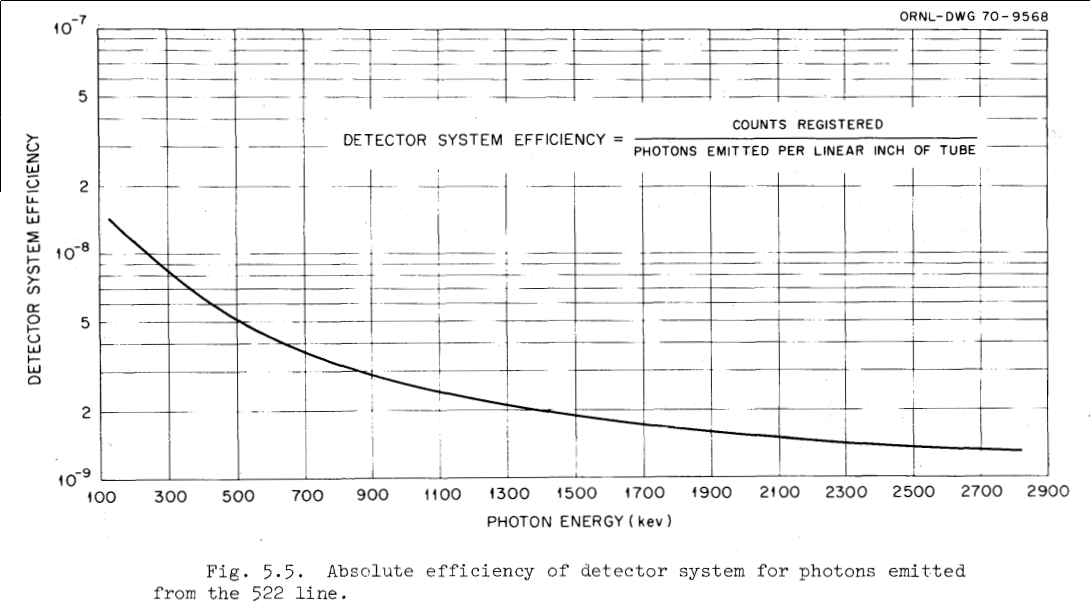
\includegraphics[width=0.8\textwidth]{Fig_5_5}
\caption{Absolute efficiency of detector system for photons emitted from the 522 line.}
\label{Fig_5_5}
\end{figure}

\begin{figure}
\centering
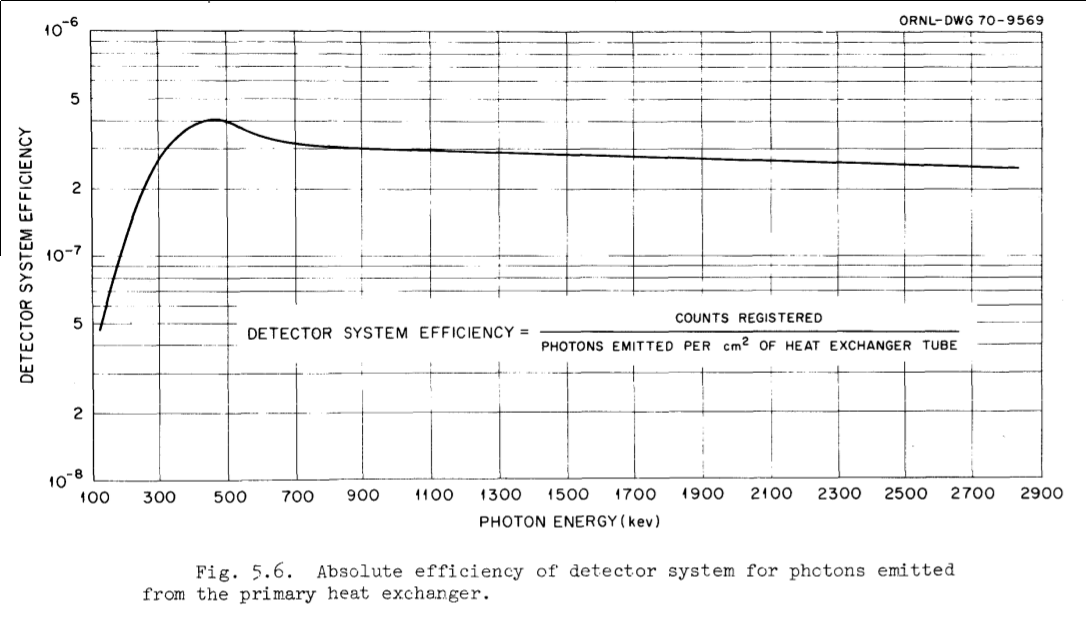
\includegraphics[width=0.8\textwidth]{Fig_5_6}
\caption{Absolute efficiency of detector system for photons emitted from the primary heat exchanger.}
\label{Fig_5_6}
\end{figure}

\section{屏蔽材料刻度}
整个实验过程中,保持探测系统的总计数率在3000-10000\ cps之间。由于源强随时间和位置的变化而变化,所有通过在探测系统和源之间插入不同的屏蔽材料来改变探测效率。在大多数情况下,用厚1/2英寸、直径7英寸的圆盘放置在PMS和准直组件之间。在激光定位时,这种圆盘容易移出。这种圆盘的材质包括铝、铜以及浸有锂的煤油。对于一些极端高放射强度水平,就得在准直体和探测器之间使用厚1/4英寸的铅盘。铅屏蔽除了有较大的衰减系数,特别对低能射线,这种材料也会和射线作用产生X射线而干扰探测。在评估不同屏蔽材料的影响时,不仅仅依赖于公布的衰减系数,也要对屏蔽圆盘做校准。使用了未屏蔽的银源和$^{226}$Ra\ 源做此事。文献提供的pb、Cu、Al、Cd和钢的衰减系数与实验值吻合;对于浸锂石蜡和换热器的陶瓷加热元件的值不得不依赖实验来获得。为所有不同的屏蔽材料绘制所谓的“屏蔽曲线”;所绘制的曲线是屏蔽系数(通常是衰减系数的倒数)在140-2500\ keV能量段的函数。

绝对效率曲线包含了实验用到的各种屏蔽材料的影响。非屏蔽效率值逐点除以屏蔽因子即可得到适当的屏蔽结果。当有多种屏蔽圆盘用到时,联合屏蔽系数计算如下:
\begin{equation}
%\label{eq:equ3}
EF_S(E)=\frac{EF_u(E)}{\prod [A_i(E)]^{N_i}}
\end{equation}
其中,$EF_S(E)$为有屏蔽体时能量E对应的效率;$EF_u(E)$为无屏蔽体时能量E对应的效率;$A_i(E)$为第i种屏蔽组件的屏蔽因子;$N_i$为第i个组件的个数。

总之,在堆主排气线上用了12种不同的屏蔽组件,而换热器的有8种,如表\ref{table_5_2}和\ref{table_5_3}所示。包含了材料屏蔽影响的效率曲线值输入到计算机分析程序中,用于评估出现的核素的绝对含量。附录C给出了不同的效率曲线。

在停堆或排料时,主要使用一些简单的铝或铜材质屏蔽体。而在不同堆功率下时,由于中子辐照和高能$\gamma$射线的存在,我们不得不用上更多屏蔽体。停堆后在不同时段用不同的屏蔽配置采集同一个位置大量的$\gamma$谱图,分析大量的沉积核素得到同样的结论;这使我们对当前使用的绝对效率曲线有一定的信心。

\begin{table}
\centering
\label{table_5_2}
\onelinecaptionsfalse
\caption{Shielding configurations employed during \protect\\
	surveys of reactor off-gas line}
\begin{tabular}[c]{ccl}
\hline
\multirow{3}{2cm}{Shielding case} & \multirow{3}{2cm}{Collimator insert 
	diameter(in.)} &  \multirow{3}{4cm}{Shielding material}\\
		\\
		\\
\hline
1  &  1/16  & 1/8\ in. steel  \\
2  &  1/8  & 1/8\ in. steel,1\ in.  Cu  \\
3  &  1/16  & 1/8\ in. steel,1\ in.  Cu,2\ in.  paraffin(Li),1/8\ in.  Cd  \\
4  &  1/8  & 1\ in. Al  \\
5  &  1/8  & None  \\
6  &  1/16  & None  \\
7  &  1/8  & 1/8\ in. Cd  \\
8  &  1/8  & 1/8\ in. Cd,1/8\ in.  steel  \\
9  &  1/16  & 1/8\ in.  Cd,1/8\ in. steel  \\
10  &  1/16  & 1/8\ in. Cd,1/8\ in.  steel,2\ in.  paraffin(Li),1/2\ in.  Pb  \\
11  &  1/16  & 1/8\ in. Cd,1/8\ in.  steel,2\ in.  paraffin(Li),1/4\ in.  Pb  \\
12  &  1/16  & 1/8\ in. Cd,1/8\ in.  steel,2\ in.  paraffin(Li) \\
\hline
\end{tabular}
\end{table}

\begin{table}
\centering
\onelinecaptionsfalse
\caption{Shielding configurations employed during \protect \\ surveys of primary heat exchanger}
\label{table_5_3}
\begin{tabular}[c]{ccl}
\hline
\multirow{3}{2cm}{Shielding case} & \multirow{3}{2cm}{Collimator insert 
	diameter(in.)} &  \multirow{3}{4cm}{Shielding material}\\
		\\
		\\
\hline
1  &  1/8  & None  \\
2  &  1/8  & 1\ in. Al \\
3  &  1/8  & 1/2\ in. Al,1/2\ in.  Cu  \\
4  &  1/8  & 1/2\ in. Al,1/2\ Cu  \\
5  &  1/8  & None  \\
6  &  1/16  & 1/8\ in. steel  \\
7  &  1/8  & 1/8\ in. Cd  \\
8  &  1/8  & 1/8\ in. Cd,1/8\ in.  steel  
\\
\hline
\end{tabular}
\end{table}

为评估1/16英寸准直插入件相对于1/8英寸的影响而做了大量的实验。在刻度实验过程中,发现使用1/16英寸插入件所降低的计数率明显高于4倍;同时单独测量时也考虑了散射影响。由于准直轴和银管中心存在轻微的错位,引起更大的误差。因此,在其他实验中,用一个轻薄活动片对准直件和探测器的末端进行微调节。相对于1/8英寸内插件,1/16英寸的屏蔽系数为9.0。这个测试做了多次验证,实验值误差在$\pm10$\%。显然,1/16英寸准直器还是不够直。


\section{MSRE中裂变气体刻度}

由于刻度所使用的刻度源来源于沉积在换热器冷却管里的放射源,计算机程序获得的结果都以这样的方式表示,包括气体。虽然气体的“等效表面沉积”模型在表示其浓度上是有效模型,但是在某些方面上根据换热器的截面体积去表示它们的浓度更有用。计算了有用体积与表面积的平均比率为0.55$cm^3/cm^2$。因此,气体的结果可以用每分钟每立方厘米的衰变数除以每分钟每平方厘米的衰变数再除以0.55。


